
%%%%%%%%%%%%%%%%%%%%%%%%%%%%%%%%%%%%%%%%%%%%%%%%%%%%%%%%%%%%%%%%%%%%%
%% This is a (brief) model paper using the achemso class
%% The document class accepts keyval options, which should include
%% the target journal and optionally the manuscript type.
%%%%%%%%%%%%%%%%%%%%%%%%%%%%%%%%%%%%%%%%%%%%%%%%%%%%%%%%%%%%%%%%%%%%%


\documentclass[journal=jacsat,manuscript=article]{achemso}
\setkeys{acs}{articletitle = true} % show titles in bibliography
%\documentclass[prb,11pt]{revtex4-1}
%\usepackage[sort&compress,numbers,super]{natbib} 
%\usepackage{achemso} 
\SectionNumbersOn 
\usepackage{wrapfig}
\usepackage{xargs}                      % Use more than one optional parameter in a new commands
\usepackage[pdftex,dvipsnames]{xcolor}  % Coloured text etc.
% 
\usepackage[colorinlistoftodos,prependcaption,textsize=tiny]{todonotes}
\newcommandx{\unsure}[2][1=]{\todo[linecolor=red,backgroundcolor=red!25,bordercolor=red,#1]{#2}}
\newcommandx{\change}[2][1=]{\todo[linecolor=OliveGreen,backgroundcolor=OliveGreen!25,bordercolor=OliveGreen,#1]{#2}}
\usepackage{amsfonts}
\usepackage{epigraph}
\setlength{\epigraphwidth}{0.7\textwidth}
%%%%%%%%%%%%%%%%%%%%%%%%%%%%%%%%%%%%%%%%%%%%%%%%%%%%%%%%%%%%%%%%%%%%%
%% Place any additional packages needed here.  Only include packages
%% which are essential, to avoid problems later. Do NOT use any
%% packages which require e-TeX (for example etoolbox): the e-TeX
%% extensions are not currently available on the ACS conversion
%% servers.
%%%%%%%%%%%%%%%%%%%%%%%%%%%%%%%%%%%%%%%%%%%%%%%%%%%%%%%%%%%%%%%%%%%%%
\usepackage[version=3]{mhchem} % Formula subscripts using \ce{}
\usepackage[T1]{fontenc}       % Use modern font encodings
\usepackage{subfig}
\usepackage{url}
\usepackage{xr} % external referecnes
\externaldocument{SI}
\renewcommand{\thepage}{S\arabic{page}}  
\renewcommand{\thesection}{S\arabic{section}}   
\renewcommand{\thetable}{S\arabic{table}}   
\renewcommand{\thefigure}{S\arabic{figure}}
\renewcommand{\theequation}{S\arabic{equation}}
\usepackage{xr} % external referecnes
\externaldocument{latent_space_of_cages}
\usepackage{natbib} 

% so S2.1
\usepackage{chngcntr}
\counterwithin{figure}{section}

% to prevent counter too large in subfigure
\usepackage{alphalph}
\renewcommand*{\thesubfigure}{%
\alphalph{\value{subfigure}}%
}%
%%%%%%%%%%%%%%%%%%%%%%%%%%%%%%%%%%%%%%%%%%%%%%%%%%%%%%%%%%%%%%%%%%%%%
%% If issues arise when submitting your manuscript, you may want to
%% un-comment the next line.  This provides information on the
%% version of every file you have used.
%%%%%%%%%%%%%%%%%%%%%%%%%%%%%%%%%%%%%%%%%%%%%%%%%%%%%%%%%%%%%%%%%%%%%
%%\listfiles

%%%%%%%%%%%%%%%%%%%%%%%%%%%%%%%%%%%%%%%%%%%%%%%%%%%%%%%%%%%%%%%%%%%%%
%% Place any additional macros here.  Please use \newcommand* where
%% possible, and avoid layout-changing macros (which are not used
%% when typesetting).
%%%%%%%%%%%%%%%%%%%%%%%%%%%%%%%%%%%%%%%%%%%%%%%%%%%%%%%%%%%%%%%%%%%%%
\newcommand*\mycommand[1]{\texttt{\emph{#1}}}

%%%%%%%%%%%%%%%%%%%%%%%%%%%%%%%%%%%%%%%%%%%%%%%%%%%%%%%%%%%%%%%%%%%%%
%% Meta-data block
%% ---------------
%% Each author should be given as a separate \author command.
%%
%% Corresponding authors should have an e-mail given after the author
%% name as an \email command. Phone and fax numbers can be given
%% using \phone and \fax, respectively; this information is optional.
%%
%% The affiliation of authors is given after the authors; each
%% \affiliation command applies to all preceding authors not already
%% assigned an affiliation.
%%
%% The affiliation takes an option argument for the short name.  This
%% will typically be something like "University of Somewhere".
%%
%% The \altaffiliation macro should be used for new address, etc.
%% On the other hand, \alsoaffiliation is used on a per author basis
%% when authors are associated with multiple institutions.
%%%%%%%%%%%%%%%%%%%%%%%%%%%%%%%%%%%%%%%%%%%%%%%%%%%%%%%%%%%%%%%%%%%%%
\author{Arni Sturluson}
\affiliation[Oregon State University]
{School of Chemical, Biological, and Environmental Engineering. Corvallis, OR, USA.}
\author{Melanie T. Huynh}
\affiliation[Oregon State University]
{School of Chemical, Biological, and Environmental Engineering. Corvallis, OR, USA.}
\author{Arthur H. P. York}
\affiliation[Oregon State University]
{School of Chemical, Biological, and Environmental Engineering. Corvallis, OR, USA.}
\author{Cory M. Simon}
%\altaffiliation{A shared footnote}
\email{Cory.Simon@oregonstate.edu}
\affiliation[Oregon State University]
{School of Chemical, Biological, and Environmental Engineering. Corvallis, OR, USA.}
%\altaffiliation{A shared footnote}
%\email{Cory.Simon@oregonstate.edu}
%\affiliation[Oregon State University]
%{School of Chemical, Biological, and Environmental Engineering. Corvallis, OR, USA.}
%\author{Carlo Carraro}
%\affiliation[University of California, Berkeley]
%{Department of Chemical and Biomolecular Engineering. Berkeley, CA, USA.}
%\altaffiliation{Current address: Some other place, Othert\"own,
%Germany}
%\author{I. Ken Groupleader}
%\altaffiliation{A shared footnote}
%\email{i.k.groupleader@unknown.uu}
%\phone{+123 (0)123 4445556}
%\fax{+123 (0)123 4445557}
%\affiliation[Unknown University]
%{Department of Chemistry, Unknown University, Unknown Town}
%\alsoaffiliation[Second University]
%{Department of Chemistry, Second University, Nearby Town}
%\author{Susanne K. Laborator}

%\affiliation[BigPharma]
%{Lead Discovery, BigPharma, Big Town, USA}
%\author{Kay T. Finally}



%%%%%%%%%%%%%%%%%%%%%%%%%%%%%%%%%%%%%%%%%%%%%%%%%%%%%%%%%%%%%%%%%%%%%
%% The document title should be given as usual. Some journals require
%% a running title from the author: this should be supplied as an
%% optional argument to \title.
%%%%%%%%%%%%%%%%%%%%%%%%%%%%%%%%%%%%%%%%%%%%%%%%%%%%%%%%%%%%%%%%%%%%%
\title[SI: Latent Space of Porous Cages]
  {Supporting Information for: Eigencages: {\color{red} Learning a latent space of porous cage molecules}}

%%%%%%%%%%%%%%%%%%%%%%%%%%%%%%%%%%%%%%%%%%%%%%%%%%%%%%%%%%%%%%%%%%%%%
%% Some journals require a list of abbreviations or keywords to be
%% supplied. These should be set up here, and will be printed after
%% the title and author information, if needed.
%%%%%%%%%%%%%%%%%%%%%%%%%%%%%%%%%%%%%%%%%%%%%%%%%%%%%%%%%%%%%%%%%%%%%
\abbreviations{IR,NMR,UV}
\keywords{American Chemical Society, \LaTeX}
\newcommand{\angstrom}{\mbox{\normalfont\AA}}

%%%%%%%%%%%%%%%%%%%%%%%%%%%%%%%%%%%%%%%%%%%%%%%%%%%%%%%%%%%%%%%%%%%%%
%% The manuscript does not need to include \maketitle, which is
%% executed automatically.
%%%%%%%%%%%%%%%%%%%%%%%%%%%%%%%%%%%%%%%%%%%%%%%%%%%%%%%%%%%%%%%%%%%%%
\begin{document}

%%%%%%%%%%%%%%%%%%%%%%%%%%%%%%%%%%%%%%%%%%%%%%%%%%%%%%%%%%%%%%%%%%%%%
%% The "tocentry" environment can be used to create an entry for the
%% graphical table of contents. It is given here as some journals
%% require that it is printed as part of the abstract page. It will
%% be automatically moved as appropriate.
%%%%%%%%%%%%%%%%%%%%%%%%%%%%%%%%%%%%%%%%%%%%%%%%%%%%%%%%%%%%%%%%%%%%%
%\begin{tocentry}
%
%Some journals require a graphical entry for the Table of Contents.
%This should be laid out ``print ready'' so that the sizing of the
%text is correct.
%
%Inside the \texttt{tocentry} environment, the font used is Helvetica
%8\,pt, as required by \emph{Journal of the American Chemical
%Society}.
%
%The surrounding frame is 9\,cm by 3.5\,cm, which is the maximum
%permitted for  \emph{Journal of the American Chemical Society}
%graphical table of content entries. The box will not resize if the
%content is too big: instead it will overflow the edge of the box.
%
%This box and the associated title will always be printed on a
%separate page at the end of the document.
%
%\end{tocentry}

%%%%%%%%%%%%%%%%%%%%%%%%%%%%%%%%%%%%%%%%%%%%%%%%%%%%%%%%%%%%%%%%%%%%%
%% The abstract environment will automatically gobble the contents
%% if an abstract is not used by the target journal.
%%%%%%%%%%%%%%%%%%%%%%%%%%%%%%%%%%%%%%%%%%%%%%%%%%%%%%%%%%%%%%%%%%%%%
%\begin{abstract}
%We use statistical thermodynamics to answer a simple question: what happens when an adsorbent is allowed to exchange gas with a rubber balloon? Richard Feynman described rubber as 'molecular spaghetti'. A statistical mechanical treatment of this molecular view of rubber captures the relationship between the pressure of gas in a rubber balloon and its radius. As a consequence of the non-monotonicity of this relationship, a gas-adsorbent-balloon system presents multi- and in-stabilities. In contrast, we show that two different adsorbents allowed to exchange gas cannot exhibit multi-stability.
%\end{abstract}

%%%%%%%%%%%%%%%%%%%%%%%%%%%%%%%%%%%%%%%%%%%%%%%%%%%%%%%%%%%%%%%%%%%%%
%% Start the main part of the manuscript here.
%%%%%%%%%%%%%%%%%%%%%%%%%%%%%%%%%%%%%%%%%%%%%%%%%%%%%%%%%%%%%%%%%%%%%
\section{Distribution of cage molecule and cavity diameters}

\begin{figure}
\centering
	\includegraphics[width=0.65\columnwidth]{../pywindow_descriptors_distn.png}
	\caption{The distribution of cage molecule diameters (red) and cage cavity diameters (blue) among the 74 cages analyzed in this work. These diameters were computed with \texttt{pywindow}. \cite{miklitz2018pywindow}.
	} \label{fig:pywindow_descriptors_distn}
\end{figure}

\newpage
\clearpage

\section{Aligning the cages before scanning} 
\label{sec:alignment_details}
We compute the $3\times 3$ moment of inertia matrix $\mathbf{I}$ of the cage, defined relative to the center of mass, and find its eigendecomposition $\mathbf{I}=\mathbf{W}\mathbf{\Lambda}\mathbf{W^T}$, with the eigenvalues arranged in a non-increasing order down the diagonal matrix $\mathbf{\Lambda}$ and the orthonormal eigenvectors in the columns of $\mathbf{W}$. Then, we transform the coordinates of the centered cage by left-multiplying by the rotation matrix $\mathbf{W^T}$. The rotated cage then possesses a diagonal moment of inertia matrix with the moments of inertia arranged in a non-increasing order down the diagonal.

\section{The data matrix $\mathbf{A}$}

\begin{figure}
\centering
	\includegraphics[width=\columnwidth]{../data_matrix_viz.png}
	\caption{An attempt at visualizing the structure of the $c \times g^3$ data matrix $\mathbf{A}$. The color depicts the magnitude of the entry of the matrix. This is an ``attempt'' because $g^3>>c$, so the data matrix $\mathbf{A}$ is wide and difficult to visualize without a longer page. Zoom in to see some structure. We remark that 10879/15625 of the columns (representing pixels in the cage cavity images) are all zeros.
	} \label{fig:data_matrix}
\end{figure}

\newpage
\clearpage

\section{The singular values of $\mathbf{A}$}

\begin{figure}
\centering
	\includegraphics[width=0.65\columnwidth]{../distn_of_svs.png}
	\caption{The distribution of the set of singular values $\sigma_1,\sigma_2, ..., \sigma_{74}$ of $\mathbf{A}$.
	} \label{fig:distn_of_svs}
\end{figure}

\newpage
\clearpage

\section{Relative error from approximating $\mathbf{A}$ as $\mathbf{A}_\nu$}

\begin{figure}
\centering
	\includegraphics[width=0.65\columnwidth]{../relative_err_with_svs.png}
	\caption{The relative error in approximating the data matrix $\mathbf{A}$ with a lower-rank-$\nu$ approximant $\mathbf{A}_\nu$ given in eqn.~\ref{eq:Anu}. The formula for the relative error as a function of $\nu$, related to the singular values of $\mathbf{A}$, is given in eqn.~\ref{eq:relative_error}.
	} \label{fig:relative_err_with_svs}
\end{figure}

\newpage
\clearpage

\section{Highlighting remaining clusters in latent cage space}

\begin{figure}[h!]
\centering
	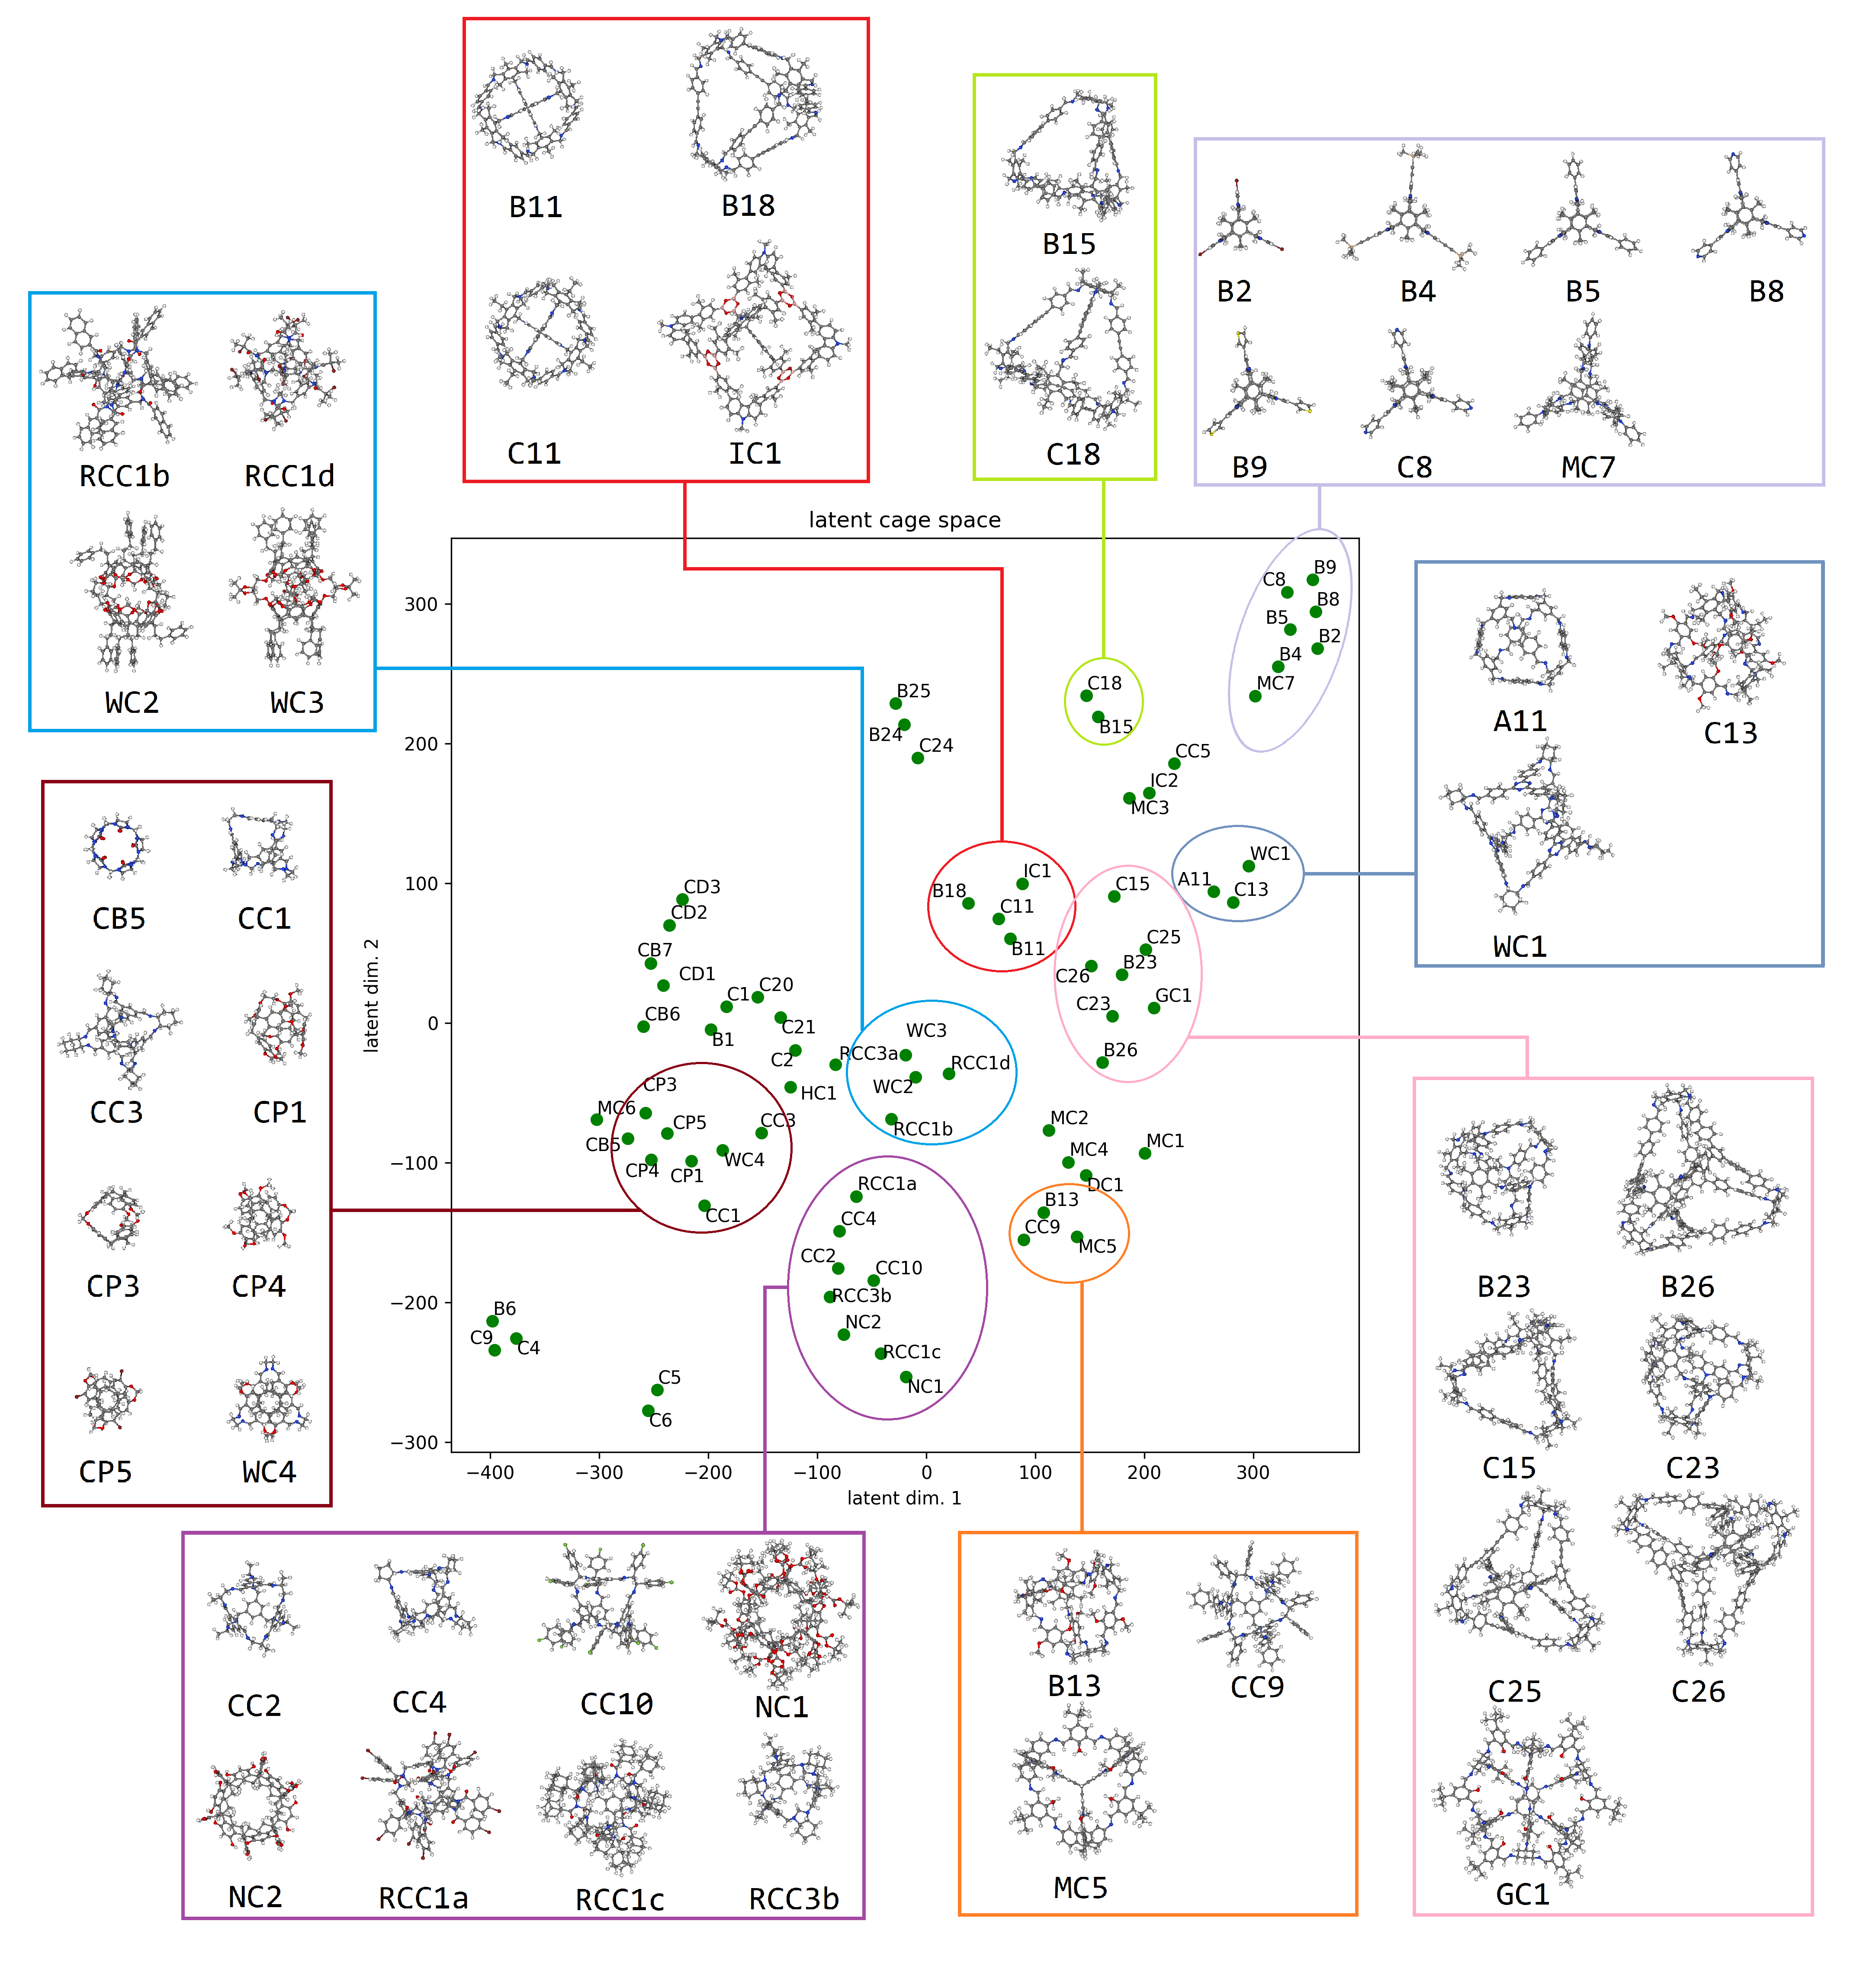
\includegraphics[width=0.9\columnwidth]{../latent_cage_space_2D_marked_SI.png}
	\caption{The latent space of cages $\mathbf{U}_\nu \mathbf{\Sigma}_\nu$ embedded into 2D by t-SNE \cite{maaten2008visualizing,wattenberg2016how}. Salient clusters are highlighted. See Fig.~\ref{fig:latent_space} for the remaining clusters.
	} \label{fig:latent_space2}
\end{figure}


\newpage
\clearpage


\section{Henry coefficient calculations} \label{sec:henrydetails} We describe more details here of the Henry coefficient calculations used to obtain the data in Fig.~\ref{fig:latent_space_S_Xe_Kr}. We model the energetics of the interaction of a gas atom (Xe, Kr, He) with the atoms of the cage as pairwise additive and with 12-6 Lennard-Jones potentials. The $\epsilon_i$ and $\sigma_i$ parameters of the Lennard-Jones potentials for atom $i$- atom $i$ interactions are taken from the Universal Force Field \cite{rappe1992uff} (cutoff radius 14~$\angstrom$). Geometric mixing rules are applied for cross-interactions. 

We placed an isolated cage molecule in an empty simulation box and took it as rigid. If $\mathbf{x} \in \mathbb{R}^3$ is the position of a gas atom in the simulation box, the molecular model described above gives us the potential energy of the gas molecule, $U(\mathbf{x})$.

Consider the isolated porous cage molecule immersed in a bath of gas; the simulation box is drawn around the porous cage molecule. Henry's law models the density of gas in the simulation box at thermodynamic equilibrium, $\rho $, as $\rho=K P$, with $K$ the Henry coefficient and $P$ the pressure of the gas. Henry's law is valid only at low surface coverage.

The Henry coefficient of a gas in the simulation box including the isolated cage molecule is given as:
\begin{equation}
K = \beta \frac{1}{|\Omega|} \int_\Omega e^{-\beta U(\mathbf{x})} d\mathbf{x},
\label{eq:K}
\end{equation} where $\beta= (k_B T)^{-1}$ is the thermodynamic beta ($T$ temperature, $k_B$ Boltzmann constant) and the integral is over the simulation box $\Omega$ (which has volume $|\Omega|$). Note that if $U(\mathbf{x})=0$, Henry's law recovers the ideal gas law $\rho = \beta P$, where $|\Omega|$ is the volume of the simulation box.

We computed the average in eqn.~\ref{eq:K} via Monte Carlo integration, i.e. Widom particle insertions \cite{frenkel2001understanding}, using 1000 Monte Carlo insertions per volume ($\angstrom^3$) of the simulation box. We used \texttt{PorousMaterials.jl} v0.1.1 \cite{PorousMaterialsJL} to compute the Henry coefficient.

\subsection{Comparing to experimental data}
By considering only an isolated cage molecule in a simulation box, as opposed to many cage molecules packed together to form a solid, we account for only the influence of the intrinsic porosity to the cage molecule on the adsorption. This is an approximation, as we are neglecting the influence of the extrinsic porosity that arises from how the cage molecules pack together to form a bulk solid. When the cage molecules pack together, the adsorption sites on the exterior of the molecule or at the cage windows can be modified depending on how the cage molecules pack together. However, when the interior of the cage molecule is the dominant adsorption site in the bulk solid, this approach may be a viable method to predict the Henry coefficient of a bulk porous cage solid.

To evaluate our crude method of considering an isolated cage molecule, Fig.~\ref{fig:expt_sim_compare} compares experimentally measured xenon and krypton adsorption isotherms in noria \cite{patil2016noria} (NC2) and CC3 \cite{chen2014separation} to the resulting Henry's law with the Henry coefficient obtained from our simulations. Fig.~\ref{fig:expt_sim_compare} shows this method yields a very good prediction of experimental Xe and Kr Henry coefficients in noria \cite{patil2016noria} (NC2), but underestimates the Henry coefficients in CC3 \cite{chen2014separation}. See Patil et. al \cite{patil2016noria} for more discussion.

\begin{figure}
\centering
	\includegraphics[width=0.4\columnwidth]{../noria_expt_sim_comparison.png}
	\includegraphics[width=0.4\columnwidth]{../CC3_expt_sim_comparison.png}
	\caption{Comparison of experimental xenon and krypton adsorption isotherms at 298 K in noria \cite{patil2016noria} and CC3 \cite{chen2014separation} to the simulated adsorption. Points show experimental data and the lines show Henry's law with the Henry coefficient taken from our simulations. The simulated Henry coefficient of He was subtracted to account for the empty space in the simulation box.
	} \label{fig:expt_sim_compare}
\end{figure}

\newpage
\clearpage

\section{Relationship of latent representation and cage molecule and cavity diameters}
Fig.~\ref{fig:first_component_captures_pore_diameter} shows that the first component of the learned latent representation of a cage is strongly correlated with its cavity diameter. 
Fig.~\ref{fig:cage_space_colored_by_diams_2D} depicts how the 2D embedding (by t-SNE) of the $\nu=23$ dimensional latent representations is correlated with the molecule diameter and cavity diameter of a porous organic cage molecule.

\begin{figure}
\centering
	\includegraphics[width=0.9\columnwidth]{../first_component_captures_pore_diameter.pdf}
	\caption{The first component of the latent representation of a cage is strongly correlated to its cavity diameter. The cavity diameter was computed by \texttt{pywindow} \cite{miklitz2018pywindow}. In the reconstruction of the 3D cavity image of a given cage, the first component of the latent representation (in the first column of $\mathbf{U}_\nu \mathbf{\Sigma}_\nu$) is the weight on the first eigencage $\mathbf{v}_1$ in the reconstruction of the 3D cage cavity image via eqn.~\ref{eq:latent_space_view}. That the first eigencage is a good descriptor of pore size is suggested by the radial symmetry of the core of the first eigencage in Fig.~\ref{fig:eigencages} that is added to the approximately radially symmetric average cage $\bar{\mathbf{c}}$ to reconstruct the 3D cage cavity image via eqn.~\ref{eq:latent_space_view}.
	} \label{fig:first_component_captures_pore_diameter}
\end{figure}


\begin{figure}
\centering
	\includegraphics[width=\columnwidth]{../cage_space_colored_by_diams_2D.png}
	\caption{The 2D embedding (by t-SNE) of the learned latent representation of the 3D cavity images contained in the rows of $\mathbf{U}_\nu \mathbf{\Sigma}_\nu$. Here, the diameter of points represents molecule diameter; color represents cavity diameter, both computed by \texttt{pywindow} \cite{miklitz2018pywindow}. Note that neighbors in latent space tend to have similar cavity and molecule diameters.
	} \label{fig:cage_space_colored_by_diams_2D}
\end{figure}

\newpage
\clearpage

\section{Relationship of latent representation and number of windows to enter cavity}

\begin{figure}
\centering
	\includegraphics[width=\columnwidth]{../cage_space_colored_by_nb_windows.png}
	\caption{The 2D embedding (by t-SNE) of the learned latent representation of the 3D cavity images contained in the rows of $\mathbf{U}_\nu \mathbf{\Sigma}_\nu$. Here, the color represents the number of windows possessed by the cage molecule. The gas molecules enter the cavity of the cage through the windows. The number of windows is computed by \texttt{pywindow} \cite{miklitz2018pywindow}. Note that cages within clusters in latent space have the same number of windows.
	} \label{fig:cage_space_colored_by_nb_windows}
\end{figure}

\newpage
\clearpage


% see viz.ipynb
\section{Visualization of the cage structures}
Larger images of the cages in Fig.~\ref{fig:cages} are shown in Fig.~\ref{fig:allcagesdetailed}.
\captionsetup[subfigure]{labelformat=empty} % get rid of a b c d
\begin{figure}[!h]
\centering
\subfloat[A11]{\includegraphics[width=0.25\columnwidth]{../all_cages/A11_final_alignment.png}}
\subfloat[B11]{\includegraphics[width=0.25\columnwidth]{../all_cages/B11_final_alignment.png}}
\subfloat[B13]{\includegraphics[width=0.25\columnwidth]{../all_cages/B13_final_alignment.png}}
\qquad
\subfloat[B15]{\includegraphics[width=0.25\columnwidth]{../all_cages/B15_final_alignment.png}}
\subfloat[B18]{\includegraphics[width=0.25\columnwidth]{../all_cages/B18_final_alignment.png}}
\subfloat[B1]{\includegraphics[width=0.25\columnwidth]{../all_cages/B1_final_alignment.png}}
\qquad
\subfloat[B23]{\includegraphics[width=0.25\columnwidth]{../all_cages/B23_final_alignment.png}}
\subfloat[B24]{\includegraphics[width=0.25\columnwidth]{../all_cages/B24_final_alignment.png}}
\subfloat[B25]{\includegraphics[width=0.25\columnwidth]{../all_cages/B25_final_alignment.png}}
\qquad
\subfloat[B26]{\includegraphics[width=0.25\columnwidth]{../all_cages/B26_final_alignment.png}}
\subfloat[B2]{\includegraphics[width=0.25\columnwidth]{../all_cages/B2_final_alignment.png}}
\subfloat[B4]{\includegraphics[width=0.25\columnwidth]{../all_cages/B4_final_alignment.png}}
\phantomcaption \end{figure}
\begin{figure}
\ContinuedFloat \centering
\subfloat[B5]{\includegraphics[width=0.25\columnwidth]{../all_cages/B5_final_alignment.png}}
\subfloat[B6]{\includegraphics[width=0.25\columnwidth]{../all_cages/B6_final_alignment.png}}
\subfloat[B8]{\includegraphics[width=0.25\columnwidth]{../all_cages/B8_final_alignment.png}}
\qquad
\subfloat[B9]{\includegraphics[width=0.25\columnwidth]{../all_cages/B9_final_alignment.png}}
\subfloat[C11]{\includegraphics[width=0.25\columnwidth]{../all_cages/C11_final_alignment.png}}
\subfloat[C13]{\includegraphics[width=0.25\columnwidth]{../all_cages/C13_final_alignment.png}}
\qquad
\subfloat[C15]{\includegraphics[width=0.25\columnwidth]{../all_cages/C15_final_alignment.png}}
\subfloat[C18]{\includegraphics[width=0.25\columnwidth]{../all_cages/C18_final_alignment.png}}
\subfloat[C1]{\includegraphics[width=0.25\columnwidth]{../all_cages/C1_final_alignment.png}}
\qquad
\subfloat[C20]{\includegraphics[width=0.25\columnwidth]{../all_cages/C20_final_alignment.png}}
\subfloat[C21]{\includegraphics[width=0.25\columnwidth]{../all_cages/C21_final_alignment.png}}
\subfloat[C23]{\includegraphics[width=0.25\columnwidth]{../all_cages/C23_final_alignment.png}}
\phantomcaption \end{figure}
\begin{figure}
\ContinuedFloat \centering
\subfloat[C24]{\includegraphics[width=0.25\columnwidth]{../all_cages/C24_final_alignment.png}}
\subfloat[C25]{\includegraphics[width=0.25\columnwidth]{../all_cages/C25_final_alignment.png}}
\subfloat[C26]{\includegraphics[width=0.25\columnwidth]{../all_cages/C26_final_alignment.png}}
\qquad
\subfloat[C2]{\includegraphics[width=0.25\columnwidth]{../all_cages/C2_final_alignment.png}}
\subfloat[C4]{\includegraphics[width=0.25\columnwidth]{../all_cages/C4_final_alignment.png}}
\subfloat[C5]{\includegraphics[width=0.25\columnwidth]{../all_cages/C5_final_alignment.png}}
\qquad
\subfloat[C6]{\includegraphics[width=0.25\columnwidth]{../all_cages/C6_final_alignment.png}}
\subfloat[C8]{\includegraphics[width=0.25\columnwidth]{../all_cages/C8_final_alignment.png}}
\subfloat[C9]{\includegraphics[width=0.25\columnwidth]{../all_cages/C9_final_alignment.png}}
\qquad
\subfloat[CB5]{\includegraphics[width=0.25\columnwidth]{../all_cages/CB5_final_alignment.png}}
\subfloat[CB6]{\includegraphics[width=0.25\columnwidth]{../all_cages/CB6_final_alignment.png}}
\subfloat[CB7]{\includegraphics[width=0.25\columnwidth]{../all_cages/CB7_final_alignment.png}}
\phantomcaption \end{figure}
\begin{figure}
\ContinuedFloat \centering
\subfloat[CC10]{\includegraphics[width=0.25\columnwidth]{../all_cages/CC10_final_alignment.png}}
\subfloat[CC1]{\includegraphics[width=0.25\columnwidth]{../all_cages/CC1_final_alignment.png}}
\subfloat[CC2]{\includegraphics[width=0.25\columnwidth]{../all_cages/CC2_final_alignment.png}}
\qquad
\subfloat[CC3]{\includegraphics[width=0.25\columnwidth]{../all_cages/CC3_final_alignment.png}}
\subfloat[CC4]{\includegraphics[width=0.25\columnwidth]{../all_cages/CC4_final_alignment.png}}
\subfloat[CC5]{\includegraphics[width=0.25\columnwidth]{../all_cages/CC5_final_alignment.png}}
\qquad
\subfloat[CC9]{\includegraphics[width=0.25\columnwidth]{../all_cages/CC9_final_alignment.png}}
\subfloat[CD1]{\includegraphics[width=0.25\columnwidth]{../all_cages/CD1_final_alignment.png}}
\subfloat[CD2]{\includegraphics[width=0.25\columnwidth]{../all_cages/CD2_final_alignment.png}}
\qquad
\subfloat[CD3]{\includegraphics[width=0.25\columnwidth]{../all_cages/CD3_final_alignment.png}}
\subfloat[CP1]{\includegraphics[width=0.25\columnwidth]{../all_cages/CP1_final_alignment.png}}
\subfloat[CP3]{\includegraphics[width=0.25\columnwidth]{../all_cages/CP3_final_alignment.png}}
\phantomcaption \end{figure}
\begin{figure}
\ContinuedFloat \centering
\subfloat[CP4]{\includegraphics[width=0.25\columnwidth]{../all_cages/CP4_final_alignment.png}}
\subfloat[CP5]{\includegraphics[width=0.25\columnwidth]{../all_cages/CP5_final_alignment.png}}
\subfloat[DC1]{\includegraphics[width=0.25\columnwidth]{../all_cages/DC1_final_alignment.png}}
\qquad
\subfloat[GC1]{\includegraphics[width=0.25\columnwidth]{../all_cages/GC1_final_alignment.png}}
\subfloat[HC1]{\includegraphics[width=0.25\columnwidth]{../all_cages/HC1_final_alignment.png}}
\subfloat[IC1]{\includegraphics[width=0.25\columnwidth]{../all_cages/IC1_final_alignment.png}}
\qquad
\subfloat[IC2]{\includegraphics[width=0.25\columnwidth]{../all_cages/IC2_final_alignment.png}}
\subfloat[MC1]{\includegraphics[width=0.25\columnwidth]{../all_cages/MC1_final_alignment.png}}
\subfloat[MC2]{\includegraphics[width=0.25\columnwidth]{../all_cages/MC2_final_alignment.png}}
\qquad
\subfloat[MC3]{\includegraphics[width=0.25\columnwidth]{../all_cages/MC3_final_alignment.png}}
\subfloat[MC4]{\includegraphics[width=0.25\columnwidth]{../all_cages/MC4_final_alignment.png}}
\subfloat[MC5]{\includegraphics[width=0.25\columnwidth]{../all_cages/MC5_final_alignment.png}}
\phantomcaption \end{figure}
\begin{figure}
\ContinuedFloat \centering
\subfloat[MC6]{\includegraphics[width=0.25\columnwidth]{../all_cages/MC6_final_alignment.png}}
\subfloat[MC7]{\includegraphics[width=0.25\columnwidth]{../all_cages/MC7_final_alignment.png}}
\subfloat[NC1]{\includegraphics[width=0.25\columnwidth]{../all_cages/NC1_final_alignment.png}}
\qquad
\subfloat[NC2]{\includegraphics[width=0.25\columnwidth]{../all_cages/NC2_final_alignment.png}}
\subfloat[RCC1a]{\includegraphics[width=0.25\columnwidth]{../all_cages/RCC1a_final_alignment.png}}
\subfloat[RCC1b]{\includegraphics[width=0.25\columnwidth]{../all_cages/RCC1b_final_alignment.png}}
\qquad
\subfloat[RCC1c]{\includegraphics[width=0.25\columnwidth]{../all_cages/RCC1c_final_alignment.png}}
\subfloat[RCC1d]{\includegraphics[width=0.25\columnwidth]{../all_cages/RCC1d_final_alignment.png}}
\subfloat[RCC3a]{\includegraphics[width=0.25\columnwidth]{../all_cages/RCC3a_final_alignment.png}}
\qquad
\subfloat[RCC3b]{\includegraphics[width=0.25\columnwidth]{../all_cages/RCC3b_final_alignment.png}}
\subfloat[WC1]{\includegraphics[width=0.25\columnwidth]{../all_cages/WC1_final_alignment.png}}
\subfloat[WC2]{\includegraphics[width=0.25\columnwidth]{../all_cages/WC2_final_alignment.png}}
\phantomcaption \end{figure}
\begin{figure}
\ContinuedFloat \centering
\subfloat[WC3]{\includegraphics[width=0.25\columnwidth]{../all_cages/WC3_final_alignment.png}}
\subfloat[WC4]{\includegraphics[width=0.25\columnwidth]{../all_cages/WC4_final_alignment.png}}
\caption{Visualizations of the structures of all 74 porous organic cage molecules analyzed in this study.
    The \texttt{.xyz} files of these cages are from Miklitz et al. and Greenaway et al. \cite{miklitz2017computational,greenaway2018high};
    see these references for the naming conventions. The cages are visualized in their centered and aligned states
    in the $[-20,20]^3$ $\angstrom$
    snapshot box in preparation for taking the 3D cage cavity image.}
\label{fig:allcagesdetailed}
\end{figure}


\newpage
\clearpage


\section{Safety statement}
As this research is all computational in nature, no unexpected or unusually high safety hazards were encountered.

\clearpage

\bibliography{bibfile}
\end{document}
